\documentclass[10pt,a4paper]{article}

\usepackage{graphicx} %graphics package

\begin{document}

\begin{figure}[ht]
	\centering
	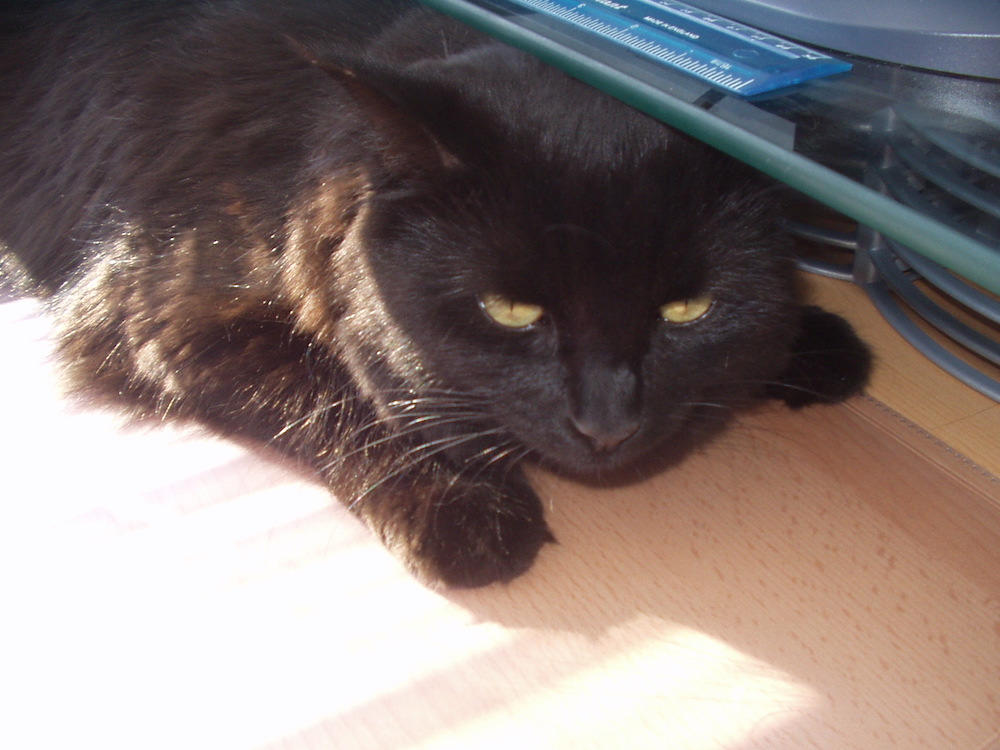
\includegraphics[width = .95\linewidth]{images/Salem.JPG}
	\caption{Salem the Cat}	
	\label{fig:figure1}
\end{figure}

\begin{table}[ht]
\begin{center}
\begin{tabular}{ p{90pt} | p{90pt} | p{90pt} | p{90pt}} 
Disney Film 				& Cat Name 	& Fur Colour 		& Favourite Food	\\ \hline
Cinderella 				& Lucifer 		& Black 			& Mice 			\\ \hline
\end{tabular}
\caption{Disney Cats}
\label{tab:table1}
\end{center}
\end{table}

Here I refer to Figure \ref{fig:figure1} and Table \ref{tab:table1}.

\end{document}

